\documentclass[slidestop,compress,mathserif]{beamer}
%\documentclass[slidestop,compress,mathserif,handout]{beamer}

%\documentclass[xcolor=dvipsnames,handout]{beamer}
%\documentclass[xcolor=dvipsnames]{beamer}

%\documentclass[handout]{beamer}

%%% To get rid of solutions on handouts:
\newcommand{\soln}[1]{\textit{\textcolor{darkGray}{#1}}}				% For slides
%\newcommand{\soln}[1]{ }	% For handouts

% to get pausing to work properly on slides
\newcommand{\hide}[1]{#1}	% For slides
%\newcommand{\hide}[1]{ }	% For handouts


%\usepackage{multicol}
\usepackage{amsfonts}
%\usepackage[pdftex,dvipsnames]{color}
\usepackage{graphicx}
\usepackage{subfigure}
%\usepackage{picinpar}
\usepackage{pifont}
\usepackage{pgf,pgfarrows,pgfnodes}
%\usepackage{wasysym,manfnt,phaistos,empheq}
\usepackage[english]{babel}
\usepackage{pgfpages}
\usepackage{natbib}
\usepackage{hyperref}
\usepackage{multimedia}
%\usepackage{amsfonts,amstext,amssymb,amsbsy,amsopn,amsthm,eucal,latexsym,mathrsfs}
\usepackage{amsmath,amsfonts,amstext,amssymb,amsbsy,amsopn,amsthm,eucal,latexsym,mathrsfs}
\usepackage{ulem}
\usepackage{setspace}
\usepackage{array}
%\usepackage{rotating}
\usepackage{multirow}
\usepackage{verbatim}
\usepackage{multicol}

\setbeamertemplate{navigation symbols}{}

%\usepackage{tikz}
%\usetikzlibrary{arrows,shapes,trees,backgrounds}


%\setbeameroption{show notes on second screen}
%\setbeameroption{show notes}
%\setbeameroption{show only notes}

\definecolor{links}{HTML}{2A1B81}
\hypersetup{colorlinks,linkcolor=,urlcolor=links}

\newtheorem*{principle}{Inscrutibility Principle}
\newtheorem*{punchline}{Punch Line}
\newtheorem{defn}{Definition}

\definecolor{Scarlet}{RGB}{140,17,17}
\definecolor{VassarRed}{RGB}{128,0,0}

% "dinglist" environment
  \renewenvironment{dinglist}[2][blue]
  {\begin{list}{\textcolor{blue}{\ding{#2}}}{}}{\end{list}}
  % Symbol definitions for these lists
  \newcommand{\DingListSymbolA}{43}
  \newcommand{\DingListSymbolB}{243}
  \newcommand{\DingListSymbolC}{224}
  \newcommand{\DingListSymbolD}{219}
  \newcommand{\DingListSymbolCheck}{52}
  \newcommand{\DingListSymbolCross}{56}


  \newenvironment{ballotenv}
{\only{%
\setbeamertemplate{itemize item}{\ding{45}}%
\setbeamertemplate{itemize subitem}{\ding{46}}%
\setbeamertemplate{itemize subsubitem}{\ding{46}}}} {}
\setbeamertemplate{itemize item}{\ding{49}}
\setbeamertemplate{itemize subitem}{\ding{47}}
\setbeamertemplate{itemize subsubitem}{\ding{47}}


%User defined colors: See colors section
\xdefinecolor{oiBlue}{rgb}{0.15, 0.35, 0.55}
\xdefinecolor{gray}{rgb}{0.5, 0.5, 0.5}
\xdefinecolor{darkGray}{rgb}{0.3, 0.3, 0.3}
\xdefinecolor{darkerGray}{rgb}{0.2, 0.2, 0.2}
\xdefinecolor{rubineRed}{rgb}{0.89,0,0.30}
\xdefinecolor{linkCol}{rgb}{0.11,0.49,0.95}	
\xdefinecolor{irishGreen}{rgb}{0,0.60,0}	
\xdefinecolor{darkturquoise}{rgb}{0.44, 0.58, 0.86}
\definecolor{lightGreen}{rgb}{0.533,0.765,0.42}
\xdefinecolor{Regalia}{HTML}{522D80}
\xdefinecolor{ClemsonOrange}{HTML}{EA6A20}

\definecolor{duke@LightGrey}{RGB}{200,200,200}\definecolor{DarkGreen}{RGB}{0,100,0}
\definecolor{Oranges}{RGB}{255,127,0}
\definecolor{LightGray}{RGB}{211,211,211}

%\setbeamertemplate{footline}{%
%  \raisebox{5pt}{\makebox[\paperwidth]{\hfill\makebox[10pt]{\scriptsize\insertframenumber}}}}

\setbeamercolor{equation background}{fg=black,bg=duke@LightGrey}
  % Boxed equation
  \newcommand{\eqbox}[2][0.6]{%
  \centerline{
  \begin{beamerboxesrounded}[lower=equation background,width=#1\hsize,shadow=true]{}
\parbox{#1\hsize}{%
      \[
        \textcolor{black} {#2}
      \]}
  \end{beamerboxesrounded}
}}

\AtBeginSection[] {
  \begin{frame}<beamer>\frametitle{Outline}
    \tableofcontents[currentsection,hideothersubsections]
  \end{frame}
}
%
%
%\AtBeginSubsection[] {
%  \begin{frame}<beamer>\frametitle{Outline}
%    \tableofcontents%[currentsection,currentsubsection]
%  \end{frame}
%}

%\usecolortheme[RGB={82,45,128}]{structure}
%\usecolortheme[RGB={162,80,22}]{structure}
\usecolortheme[RGB={128,0,0}]{structure}
\usetheme[secheader]{Boadilla}
%\usetheme[height=7mm]{Rochester}
%\usetheme{Copenhagen}
%\usetheme{Antibes}
%\usecolortheme{seahorse}
%\usecolortheme{crane}
%\usecolortheme{rose}
%\usefonttheme[onlylarge]{structurebold}
%\usefonttheme[onlymath]{serif}



\def\diag{{\rm diag}}


\def\E{\mathbb{E}}
\def\Prob{\mathbb{P}}
\def\argmin{{\rm argmin}}
\def\argmax{{\rm argmax}}
\def\Def{\stackrel{def}{=}}


\newtheorem{assumption}{Assumptions}
\newtheorem*{proposition}{Proposition}
\newtheorem*{remark}{Remark}



%\setbeamercolor{disc title}{bg=oiBlue!40!white!60,fg=blue}
\setbeamercolor{disc body}{bg= Regalia!20!white!80,fg= Regalia!80!black!90}

\setbeamercolor{clicker ungraded title}{bg=irishGreen!80!white!50,fg=irishGreen!30!black!90}
\setbeamercolor{clicker ungraded body}{bg=irishGreen!20!white!80,fg=irishGreen!30!black!90}

\setbeamercolor{clicker review title}{bg=gray!80!white!80,fg=oiBlue!80!black!90}
\setbeamercolor{clicker review body}{bg=gray!30!white!90,fg=oiBlue!80!black!90}

\setbeamercolor{code body}{bg=gray!20!white!80,fg=black}


% Custom commands
\newcommand{\degree}{\ensuremath{^\circ}}
\newcommand{\Note}[1]{
\rule{2.5cm}{0.25pt} \\ \textit{\scriptsize {\textcolor{rubineRed}{Note:} \textcolor{gray}{#1}}}}
\newcommand{\ct}[1]{
\vfill
{\tiny #1}}
\newcommand{\Remember}[1]{\textit{\scriptsize{\textcolor{orange}{Remember:} \textcolor{gray}{#1}}}}
\newcommand{\red}[1]{\textit{\textcolor{rubineRed}{#1}}}
\newcommand{\pink}[1]{\textit{\textcolor{rubineRed!90!white!50}{#1}}}
\newcommand{\green}[1]{\textit{\textcolor{irishGreen}{#1}}}
\newcommand{\webURL}[1]{\urlstyle{same}\textit{\textcolor{linkCol}{\url{#1}}} }
\newcommand{\webLink}[2]{\href{#1}{\textcolor{linkCol}{{#2}}}}
\newcommand{\mail}[1]{\href{mailto:#1}{\textit{\textcolor{linkCol}{#1}}}}
\newcommand{\hl}[1]{\textit{\textcolor{oiBlue}{#1}}}
\newcommand{\hlGr}[1]{\textit{\textcolor{lightGreen}{#1}}}
\newcommand{\mathhl}[1]{\textcolor{oiBlue}{\ensuremath{#1}}}
\newcommand{\ex}[1]{\textcolor{blue}{{{\small (#1)}}}}
\newcommand{\disc}[1]{
\begin{beamerboxesrounded}[shadow = true, lower = disc body, upper = disc title]{}
#1
\end{beamerboxesrounded}
}

\newcommand{\cl}[1]{
\begin{beamerboxesrounded}[shadow = true, lower = clicker ungraded body, upper = clicker ungraded title]{Question}
$\:$ \\
#1
\end{beamerboxesrounded}
}

\newcommand{\clR}[1]{
\begin{beamerboxesrounded}[shadow = true, lower = clicker review body, upper = clicker review title]{\red{Review question} }
$\:$ \\
#1
\end{beamerboxesrounded}
}

\newcommand{\formula}[2]{
\begin{beamerboxesrounded}[shadow = true, lower = white, upper = clicker review body]{#1}
#2
\end{beamerboxesrounded}
$\:$ \\
}

\newenvironment{twocol}[4]{
\begin{columns}[c]
\column{#1\textwidth}
#3
\column{#2\textwidth}
#4
\end{columns}
}


\newenvironment{slot}[2]{
\begin{array}{c}
\underline{#1} \\
#2
\end{array}
}

\newcommand{\pr}[1]{
\left( #1 \right)
}

\newcommand{\solnMult}[1]{
\item[] \vspace{-0.59cm}
\only<beamer| beamer:1>{\item #1}
\soln{\only<2->{\item \red{#1}}}
}

%\newcommand{\codechunk}[1]{
%\begin{beamerboxesrounded}[shadow = true, lower = code body]{}
%{\small #1}
%\end{beamerboxesrounded}
%}

% Change margin

\newenvironment{changemargin}[2]{%
\begin{list}{}{%
\setlength{\topsep}{0pt}%
\setlength{\leftmargin}{#1}%
\setlength{\rightmargin}{#2}%
\setlength{\listparindent}{\parindent}%
\setlength{\itemindent}{\parindent}%
\setlength{\parsep}{\parskip}%
}%
\item[]}{\end{list}}

% Footnote

\long\def\symbolfootnote[#1]#2{\begingroup%
\def\thefootnote{\fnsymbol{footnote}}\footnote[#1]{#2}\endgroup}

% Commands from the book
\newenvironment{data}[1]{\texttt{#1}}{}
\newenvironment{var}[1]{\texttt{#1}}{}
\newenvironment{resp}[1]{\texttt{#1}}{}






%%%%%%%%%%%%%%%%%%%%%%%%%%%%%%%%%%%%%%%%%%%%%%%%%%%%%%%%%%%%%%%%%%%%%%%%%%%%%%%%%%%%%%%%%%%%%%%

\title[Chapter 4 part 1]{Chapter 4 part 1}
\subtitle{Discrete Random Variables}

%%%%%%%%%%%%%%%%%%%%%%%%%%%%%%%%%%%%%%%%%%%%%%%%%%%%%%%%%%%%%%%%%%%%%%%%%%%%%%%%%%%%%%%%%%%%%%%


\author[Jingchen (Monika) Hu] % (optional, use only with lots of authors)
{Jingchen (Monika) Hu}
% - Give the names in the same order as the appear in the paper.
% - Use the \inst{?} command only if the authors have different
%   affiliation.

\institute[Vassar] % (optional, but mostly needed)
{Vassar College}
% - Use the \inst command only if there are several affiliations.
% - Keep it simple, no one is interested in your street address.

\date[MATH 241] % (optional, should be abbreviation of conference name)
{MATH 241}
% - Either use conference name or its abbreviation.
% - Not really informative to the audience, more for people (including
%   yourself) who are reading the slides online

\subject{MATH 241}
% This is only inserted into the PDF information catalog. Can be left
% out.



% If you wish to uncover everything in a step-wise fashion, uncomment
% the following command:

%\beamerdefaultoverlayspecification{<+->}


\begin{document}




%%%%%%%%%%%%%%%%%%%%%

% Title Page

\begin{frame}%[plain]
\titlepage
\end{frame}

%%%%%%%%%%%%%%%%%%%%%
%\addtocounter{framenumber}{-1}
%
%\begin{frame}\frametitle{Annoucement}
%
%\begin{itemize}
%\item HW3: \red{due now!}
%\item HW4: \red{due Tuesday, Sept 30th}
%\end{itemize}
%
%
%\end{frame}
%
%


%%%%%%%%%%%%%%%%%%%%%
\begin{frame}{Outline}
%\tableofcontents[hideallsubsections,pausections]
\tableofcontents[hideallsubsections]
\end{frame}



%%%%%%%%%%%%%%%%%%%%%%%%%%%%%%%%%%%%%%%%%%
\section{Discrete random variables}
%%%%%%%%%%%%%%%%%%%%%%%%%%%%%%%%%%%%%%%%%%
\begin{frame}
\frametitle{Random Variables}

\begin{defn}
\hl{Random Variable} $X$ is a real-valued  function on the sample space $S$.
\end{defn}

%\vspace{5mm}
\pause
Example: If $S = \{a = (a_1,a_2): 1\leq a_1, a_2 \leq 6\}$ is the 36 element space resulting from rolling two fair six-sided dice, then the following are all random variables
\begin{align*}
X(a) &= a_1 \\
Y(a) &= |a_1-a_2| \\
Z(a) &= a_1+a_2
\end{align*}


\pause
\begin{itemize}
\item Random variable is a number associated with a random experiment.
\item Random variables are in essence a fancy way of describing an event, e.g.
\[P(X=1) = 1/6\]

\end{itemize}
\end{frame}



%%%%%%%%%%%%%%%%%%%%%%%%%%%%%%%%%%%%%%%%%%
\begin{frame}

\disc{Example: a coin is flipped until a head is obtained. The flips are independent and each one has probability $p$ of heads.
Let the random variable $X$ denote the number of flips until a head is obtained.
}

\pause
\begin{align*}
P(X = 1) & = P(\text{H}) = p\\
P(X = 2) & = P(\text{TH}) = (1-p)p\\
P(X = 3) & = P(\text{TTH}) = (1-p)^2 p\\
 \cdots & \cdots \\
P(X = n) & = P(\text{TT} \cdots \text{TH}) = (1-p)^{n-1}p \\
 \cdots & \cdots
\end{align*}

\end{frame}


%%%%%%%%%%%%%%%%%%%%%%%%%%%%%%%%%%%%%%%%%%
\begin{frame}\frametitle{Cumulative distribution function (cdf)}
\begin{defn}
For a random variable $X$, the function $F$ defined by
\[ F(x) = P(X \leq x), \quad  -\infty < x < \infty \]
is called the \hl{cumulative distribution function} of $X$.
\end{defn}

\pause
Note that
\begin{itemize}
\item Capital $X$: random variable
\item Little $x$: a real-valued number
\item $\leq$: smaller than or equal to
\end{itemize}

\pause
In the previous coin flipping example,
\[F(n) = P(X \leq n) = \sum_{i=1}^n (1-p)^{i-1} p = \frac{[1-(1-p)^n]p}{1-(1-p)} = 1- (1-p)^n\]

\end{frame}

%%%%%%%%%%%%%%%%%%%%%%%%%%%%%%%%%%%%%%%%%%
\begin{frame}\frametitle{Properties of the cdf (Ch 4.10)}

\begin{itemize}
\item $P(a < X \leq b) = F(b) - F(a)$, for all $a<b$

\pause
\item $P(X < b)$ does not necessary equal to $P(X\leq b)$.
\end{itemize}

\pause
\begin{enumerate}
\item $F(x)$ is a non-decreasing function; i.e., if $x_1 < x_2$, then
\[F(x_1) \leq F(x_2)\]

\pause \vspace{-0.5cm}
\item \[ \lim_{x \rightarrow \infty} F(x) = 1 \Longleftrightarrow P(X \leq \infty) = 1\]

\pause \vspace{-0.5cm}
\item \[ \lim_{x \rightarrow -\infty} F(x) = 0 \Longleftrightarrow P(X > -\infty) = 1\]

\pause \vspace{-0.1cm}
\item $F(x)$ is right continuous; i.e., for any decreasing sequence $\{x_n: n = 1, 2, \ldots \}$ that converges to $x$,
\[ \lim_{n\rightarrow \infty}F(x_n) = F(x)\Longrightarrow \lim_{n\rightarrow \infty}P(X \leq x + \frac{1}{n}) = P(X \leq x)\]
\end{enumerate}


\end{frame}



%%%%%%%%%%%%%%%%%%%%%%%%%%%%%%%%%%%%%%%%%%
\begin{frame}{The cdf tells us everything about a random variable $X$}

\vspace{-0.5cm}
\begin{center}
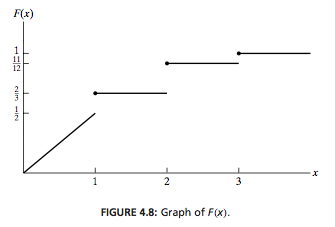
\includegraphics[scale=0.7]{figures/cdf}
\end{center}

\pause \vspace{-0.5cm}
\twocol{0.5}{0.5}
{
\begin{itemize}
\item $P(X \leq 0.5) = 0.5 \times \frac{1/2}{1} = 0.25$
\pause
\item $P(X > 2) = 1 - P(X \leq 2) = \frac{1}{12}$
\end{itemize}
}
{
\pause
\begin{itemize}
\item $P(X < 1) = 0.5, P(X \leq 1) = \frac{2}{3}$
\pause
\item $P(X = 1) = P(X \leq 1)$\\ $- P(X < 1) = \frac{2}{3} - \frac{1}{2} = \frac{1}{6}$
\end{itemize}
}

\end{frame}


%%%%%%%%%%%%%%%%%%%%%%%%%%%%%%%%%%%%%%%%%%
\begin{frame}\frametitle{Discrete random variables}
\begin{defn}
\begin{dinglist}{\DingListSymbolA}
\item A random variable $X$ that can take on at most a countable number of possible values is a
\hl{discrete random variable}.
\pause
\item For a discrete random variable $X$, we define the \hl{probability mass function} (pmf) by
\[ p(x) = P(X = x) \]
\end{dinglist}
\end{defn}
\vspace{-0.1cm}
Note: pmf is also written as $f(x)$.
\pause

Examples of discrete random variable
\begin{itemize}
\item Flip a coin 10 times, $X = $ number of heads.\\
$X$ can be $0, 1, 2, \ldots, 10$, finite. $\Longrightarrow$ discrete random variable.

\pause
\item $X =$ number of your ex boyfriends / girlfriends.\\
$X$ can be $0, 1, 2, \ldots, \infty$, countable. $\Longrightarrow$ discrete random variable.

\pause
\item $X=$ a random number in $[0, 1]$ generated by computer\\
$X$ can anything in $[0, 1]$, uncountable. $\Longrightarrow$ not discrete random variable.


\end{itemize}


\end{frame}


%%%%%%%%%%%%%%%%%%%%%%%%%%%%%%%%%%%%%%%%%%
\begin{frame}\frametitle{pmf and cdf}
\begin{itemize}
\item For a discrete random variable $X$, there exists a countable sequence $x_1, x_2, \ldots$, such that
\begin{align*}
p(x_i) > 0 & \quad\text{ for } i = 1, 2, \ldots\\
p(x) = 0 & \quad\text{ for all other values of }x
\end{align*}
\pause
and
\[ \sum_{i=1}^\infty p(x_i) = 1 \]

\pause
\item Relationship between pmf and cdf (for discrete random variable)
\[ F(a) = \sum_{\text{all } x \leq a} p(x)\]

\item If we know pmf, we can compute cdf. And vice versa.

\end{itemize}

\end{frame}

%%%%%%%%%%%%%%%%%%%%%%%%%%%%%%%%%%%%%%%%%%
\begin{frame}%\frametitle
X has a pmf given by
\[p(1) = \frac{1}{4},\ p(2) = \frac{1}{2},\ p(3) = \frac{1}{8},\ p(4) = \frac{1}{8} \]

\twocol{0.4}{0.6}
{
\pause
\begin{center}
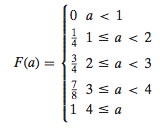
\includegraphics[scale = 0.8]{figures/eg_cdf}
\end{center}
}
{
\pause
\begin{center}
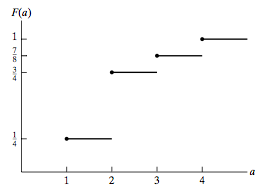
\includegraphics[scale = 0.75]{figures/eg_cdf2}
\end{center}
}


\end{frame}

%%%%%%%%%%%%%%%%%%%%%%%%%%%%%%%%%%%%%%%%%%
\begin{frame}\frametitle{Recap}

Random Variable
\begin{itemize}
\item Random Variable $X$ is a real-valued  function on the sample space $S$.
\[ X: S \longrightarrow \mathbb{R}\]

\item Cumulative distribution function (cdf)
\[ F_X(x) = P(X \leq x), \quad \text{for any } x \in \mathbb{R} \]
\end{itemize}

\pause
Discrete random variable
\begin{itemize}
\item can only take at most a countable number of possible values.
\item probability mass function (pmf)
\[ p_X(x) = P(X = x) \]
\end{itemize}
\pause
\vspace{-0.3cm}
\twocol{0.5}{0.5}
{
\begin{itemize}
\item $\sum_{i=1}^{\infty} p(x_i) = 1$
\end{itemize}
}
{
\begin{itemize}
\item $F(a) = \sum_{\text{all } x \leq a} p(x)$
\end{itemize}
}



\end{frame}

%%%%%%%%%%%%%%%%%%%%%%%%%%%%%%%%%%%%

%%%%%%%%%%%%%%%%%%%%%%
%\begin{frame}{Outline}
%%\tableofcontents[hideallsubsections,pausections]
%\tableofcontents[hideallsubsections]
%\end{frame}


%%%%%%%%%%%%%%%%%%%%%%%%%%%%%%%%%%%%%%%%%%
\section{Expectation}
%%%%%%%%%%%%%%%%%%%%%%%%%%%%%%%%%%%%%%%%%%
\begin{frame}
\frametitle{Expected value}
\begin{defn}
The \hl{expected value} (or \hl{mean}) of a \underline{discrete random variable} is defined as
\[E[X] = \sum_{x: p(x) > 0} x\cdot P(X = x)= \sum_{x: p(x) > 0} x p(x)\]
\end{defn}

\pause
\begin{itemize}
\item $E[X]$ is a weighted average of the possible values $x$ that $X$ can take on,
each value being weighted by the probability $p(x) $.
\end{itemize}

\pause\vspace{0.5cm}
\twocol{0.2}{0.7}
{

\includegraphics[width = 0.5\textwidth]{figures/joke1}

\includegraphics[width = 0.5\textwidth]{figures/joke2}
}
{
When she told me I was average, \\
she was just being mean.
}


\end{frame}

%%%%%%%%%%%%%%%%%%%%%%%%%%%%%%%%%%%%%%%%%%
\begin{frame}

\disc{Example: $X$ is the outcome when we roll a 4-sided fair die. Find $E[X]$.}
%\invisible{
\pause
\[ p(1) = p(2) = p(3) = p(4) = \frac{1}{4} \]
\[ E[X] = 1\times \frac{1}{4} + 2\times \frac{1}{4} + 3\times \frac{1}{4} + 4\times \frac{1}{4} = 2.5 \]
%}


\end{frame}



%%%%%%%%%%%%%%%%%%%%%%%%%%%%%%%%%%%%%%%%%%
\begin{frame}\frametitle{Expectation of a function of a random variable}
\begin{itemize}
\item If $X$ is a discrete random variable, and $g$ is a real-valued function then the expectation (or expected value) of $Y = g(X)$ is
\[ E[g(X)] = \sum_{x: p_X(x) > 0} g(x) \cdot p_X(x) \]
\end{itemize}


\end{frame}

%%%%%%%%%%%%%%%%%%%%%%%%%%%%%%%%%%%%%%%%%%
\begin{frame}
\disc{
$X$ is a discrete random variable with pmf
\begin{center}
\begin{tabular}{c | c | c | c}
$x$			& $-1$			& $0$ 			& $1$			\\
\hline
$p_X(x)$	&$1/4$			&$1/2$			& $1/4$ 			\\
\end{tabular}
\end{center}
$Y = X^2$.
Compute $E[Y]$.
}

%\invisible{
\pause
\begin{align*}
E[Y] & = \sum_{\text{all }x} x^2 \cdot p_X(x)\\
& = (-1)^2 \times \frac{1}{4} + 0^2 \times \frac{1}{2} + 1^2 \times \frac{1}{4}\\
& = \frac{1}{2}
\end{align*}

%}

\end{frame}

%%%%%%%%%%%%%%%%%%%%%%%%%%%%%%%%%%%%

\begin{frame}
\frametitle{Properties of expected values}

If $a$ and $b$ are constants, then
\[ E[aX+b] = a E[X] + b \]


\begin{itemize}
\item Holds for all random variable $X$ (not necessary discrete random variable).
\pause \vspace{2mm}
\item Proof for discrete random variable: let $g(X) = aX + b$
\end{itemize}

\end{frame}

%%%%%%%%%%%%%%%%%%%%%%%%%%%%%%%%%%%%

\begin{frame}%\frametitle{}
Special cases of linear transformation $ E[aX+b] = a E[X] + b $
\begin{itemize}
\item constant factor \[ E[aX] = a E[X] \]

\vspace{2cm}
\item constant \[ E[b] = b \]
\end{itemize}

\end{frame}
%%%%%%%%%%%%%%%%%%%%%%%%%%%%%%%%%%%%


%%%%%%%%%%%%%%%%%%%%%%%%%%%%%%%%%%%%%%%%%%
\begin{frame}\frametitle{Recap}

Expectation $\mu$
\begin{itemize}
\item \textbf{For discrete random variable}: $E[X] = \sum_{\text{all } x} x \cdot p(x)$
\item \textbf{Functions}: $E[g(X)] = \sum_{\text{all }x} g(x)~p(x)$
\vspace{2mm}
\item \textbf{Indicators}: $E[\delta_A] = P(A)$ where $\delta_A$ is an indicator function
\item \textbf{Linear function}: $E[aX + b] = aE[X] + b$
\item \textbf{Constants}: $E[c] = c$ if $c$ is constant
\end{itemize}

\pause
For two random variable's $X$ and $Y$
\[E[X + Y] = E[X] + E[Y]\]

\end{frame}

%%%%%%%%%%%%%%%%%%%%%%%%%%%%%%%%%%%%

%%%%%%%%%%%%%%%%%%%%%%
%\begin{frame}{Outline}
%%\tableofcontents[hideallsubsections,pausections]
%\tableofcontents[hideallsubsections]
%\end{frame}


\end{document}
